% The variation in words used across subdomains suggests that people often describe our stimuli in terms of subdomain-specific \textit{part concepts}. 
The results so far suggest that people invoke subdomain-specific part concepts when describing the objects in our stimulus set, such as \texttt{knobs} and \texttt{drawers}, or \texttt{windows} and \texttt{doors}.
% Tasked with describing a highly-structured set of related objects, participants readily pick out and name part concepts like \textit{knobs} and \textit{drawers}, or 
% \textit{windows} and \textit{doors}. 
% But how do they choose this particular lexicon: what determines \textit{how many} and \textit{which} part concepts, they name?
What accounts for observed preferences for this lexicon --- how many and which part concepts do people have names for?

In this section, we formalize this problem as search over a space of possible concept libraries that can be used to represent each subdomain. We introduce a \textit{library abstraction} procedure used to populate this hypothesis space with libraries containing parts at varying levels of complexity, based on the hierarchical visual structure inherent within each subdomain. We then use introduce a \textit{library-to-vocabulary alignment} model from the statistical machine translation literature that measures how well programs written in each library predict the language people use to describe objects in each subdomain.
% Using these tools, we can formalize a hypothesis linking \textit{lexical choice} to a trade-off in \textit{conceptual representation}: we propose 
These tools allow us to evaluate a hypothesis concerning the relationship between concept representations and lexical choice --- in particular, that people favor a lexicon that enables concise descriptions of objects on average while also minimizing the size of the concept library.

% The variation in vocabularies used across subdomains suggests that participants represented objects in our dataset using higher-level of abstractions than the library of base primitives used to define them. N

%% SEARCH OVER LIBRARIES
% In this section, we turn from instance-level descriptions to subdomains: how do speakers choose a \textit{lexicon} of words and part concepts to describe the subdomain as a whole?

% Building on our modeling approach from Part I -- which correlates individual stimulus instructions and stimulus programs using a \textit{description length} metric -- we introduce two analogous modeling techniques: a \textit{DSL abstraction} procedure, which allows us to construct higher-order DSLs based on subdomain part structure; and a \textit{DSL-vocabulary alignment model}, used to measure correspondences between entire vocabularies and program DSLs.

% We use this extended model to formalize a hypothesis that links linguistic vocabularies to latent \textit{subdomain-level} structure: we expect that speakers tailor their vocabularies across the subdomain to reflect both the representational cost of \textit{individual stimuli} (based on individual program description lengths) and of the \textit{subdomain as a whole} (based on the size of the DSL containing all program concepts across the subdomain.)ca


\subsection{Methods}
\paragraph{Defining a hypothesis space over graphics libraries} 

\begin{figure}[t]
  \begin{center}
  \includegraphics[width=0.99\linewidth]{figures/lax_libraries_gradient.pdf} % swap to figures/lax_libraries.pdf to remove bars
  \caption{Graphics libraries were defined by progressively adding subroutines at higher levels of abstraction, resulting in more efficient expression of any particular program at the expense of a larger library.}
  \label{fig:library_gallery}
  \end{center}
\end{figure}

% By design, the generative procedures for each subdomain described in Part I are highly structured: stimuli are constructed through the hierarchical combination of increasingly complex parts. 
By design, the objects in our stimulus set are highly structured, having been generated through the hierarchical combination of increasingly complex parts.
However, the corresponding graphics programs that recreate them were written using a concept library containing only the base primitives ($\mathcal{L}_{base}$): \texttt{blocks} and \texttt{lines}.
% However, the corresponding \textit{graphics programs} they produce (and whose lengths we measure in Part I) are written in the base library $\mathcal{L}_{base}$ of low-level primitives (\textit{blocks} and simple \textit{curves}) shared across the domain. 
As a consequence, these programs are maximally verbose: they must compose many individual blocks to represent a \texttt{door}, let alone an entire \texttt{house}; and many individual lines to represent a polygon like a \texttt{hexagon}, let alone a complex \texttt{wheel}. 

To represent more complex shapes, we define higher-order graphics libraries that augment the initial set of base primitives with \textit{program subroutines} (Fig.~\ref{fig:library_gallery}) that encapsulate part structure (e.g., a subroutine for generating an entire \texttt{roof}).\footnote{Our approach to defining these higher-order libraries is analogous to the automated program library learning methods in \shortcite{ellis2020dreamcoder, tian2020learning, mccarthy2021learning, wang2021learning,wong2021leveraging}, which discover subroutines from a dataset containing programs that often correspond qualitatively to domain-relevant concepts.}
We constructed these libraries by abstracting out the nested, parametric functions used to generate each subdomain. 
In our experiments, we evaluate three libraries ($\mathcal{L}_1$, $\mathcal{L}_2$, and $\mathcal{L}_3$), each containing subroutines that build recursively on those at the previous level to yield increasingly complex visual parts.
% characterized by three levels of increasing abstraction. 
% Components in successively higher-order libraries build recursively on those at the previous level. 
For instance, $\mathcal{L}_1$ contains subroutines that abstract directly over the base library (e.g., from \texttt{lines} to \texttt{polygons}); and $\mathcal{L}_2$ contains subroutines that abstract additionally over those in $\mathcal{L}_1$ (e.g., \texttt{polygons} to \texttt{rings of polygons}). 
A given program $\pi_{\mathcal{L}_{base}}$ written in the base library can therefore be expressed equivalently---and more concisely---as $\pi_{\mathcal{L}_{i}}$ in one of the higher-order libraries. 
It is worth noting that higher-order libraries are thus defined \textit{cumulatively}:
% , reflecting the recursive nature of how each new abstraction layer is defined: 
$\mathcal{L}_1$ contains the new subroutines \textit{plus} the initial set of primitives in $\pi_{\mathcal{L}_{base}}$; and $\mathcal{L}_2$ contains even higher-order subroutines \textit{plus} all of the concepts in $\mathcal{L}_1$.

% GG: I've combined this plus another paragraph into the above
% We can, however, define \textit{higher-order libraries} that abstract out the nested, parametric functions used to generate each subdomain. Formally, these higher-order libraries rewrite the program for each stimulus in terms of concise program abstractions: chunked subroutines representing repeated part structure (such as \textit{wheel} or \textit{roof} components) shared across a given subdomain
% (see Fig. \ref{fig:library_gallery}). Each of these libraries represents a \textit{hypothesis} about a possible part decomposition for the subdomain: by constructing several such libraries, we can ask which best predicts the words people actually use.

% \footnote{Our approach to defining these higher-order libraries is analogous to the automated program library learning methods in \shortcite{ellis2020dreamcoder, tian2020learning, mccarthy2021learning, wang2021learning}, which discover subroutines from a dataset containing programs that often correspond qualitatively to domain-relevant concepts.}
% Our top-down library extraction procedure is analogous to the automated, bottom-up \textit{program library learning} methods in \shortcite{ellis2020dreamcoder, tian2020learning, mccarthy2021learning}, which discover subroutines from a dataset of programs that often correspond qualitatively to domain-relevant concepts.
% % However, with access to each subdomain's hierarchical generation procedure, we can construct these DSLs directly.
% However, in this work, we chose to construct libraries manually, allowing us to consider a wide range of abstraction levels while maintaining a high degree of fidelity to the procedures by which the stimuli were originally generated.


\paragraph{Library-to-vocabulary alignment model}
For each subdomain, the set of libraries $\{\mathcal{L}_{base}, \mathcal{L}_1, \mathcal{L}_2, \mathcal{L}_3\}$ specifies a hypothesis space of alternative representations at differing levels of abstraction. We can now ask: which of these libraries best corresponds to the lexicon people use for each subdomain?

% We formalize this notion of lexical correspondence with a \textit{vocabulary-DSL alignment metric} that leverages token-token statistical alignment models used to relate parallel language datasets in machine translation. Here, we use these models to derive an aggregate metric of how closely program components in a given DSL co-occur with words across each subdomain.

We formalize this notion of lexical correspondence with a \textit{library-to-vocabulary alignment metric} that reflects how closely the concepts in a given library co-occur with words across each subdomain. 
To compute this metric, we leverage IBM Model 1 \shortcite{brown1993mathematics}, a standard machine translation model which can be fit to paired programs and instructions to estimate token-token translation probabilities $P(w|\rho)$ for each word $w \in W$ in the linguistic vocabulary and program component $\rho \in \mathcal{L}$ in the library. 
For each subdomain, we evaluate each library $\mathcal{L}_i$ using a cross-validation scheme (with batches of $n=5$ held out stimuli). 
We fit the model to all but the held-out stimuli and evaluate the \textit{mean per-word log-likelihood} for each held out instruction given its program in library $\mathcal{L}_i$. 
We use \textit{mean token log-likelihood}, which correlates monotonically with negative {perplexity} \shortcite{wu2016google}, to normalize for instruction lengths. As in Part I, we consider only the language provided in the \textit{what} phrases for each stimulus.

% \begin{figure*}[!ht]
%   \begin{center}
%   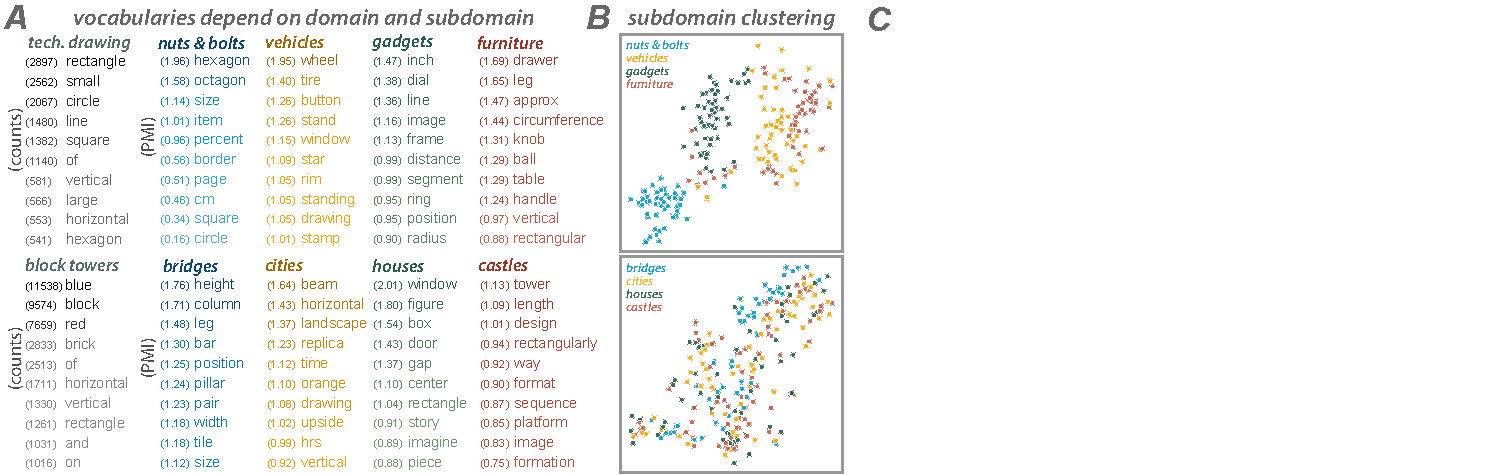
\includegraphics[width=1.0\linewidth]{figures/lax_vocabularies.pdf}
%   \caption{(A) Word counts for domain. PMI for subdomains. (B) Clustering of word-count vectors shows more distinct language across subdomains of technical drawings than of block towers. Each point is a participant, each of whom described items in a single subdomain. (C) }
%   \label{fig:vocabulary_gallery}
%   \end{center}
% \end{figure*}


\begin{figure*}[ht!]
  \begin{center}
  \includegraphics[width=0.99\linewidth]{figures/lax_library_costs.pdf}
  \caption{Relationship between concept libraries \{$L_{base}$, $\mathcal{L}_1$, $\mathcal{L}_2$, and $\mathcal{L}_3$\} (x-axis); combined library size and average program length in that library (dashed); and library-to-vocabulary alignment (solid).}\label{fig:perplexity-length}
  \end{center}
\end{figure*}

\subsection{Results}
\paragraph{Each library represents a different trade-off between compressing objects and minimizing library size} 
% The set of libraries we consider defines a hypothesis space over sets of concepts that participants could be using to represent the parts of objects in a subdomain. 
% ($\{\mathcal{L}_{base}, \mathcal{L}_1, \mathcal{L}_2, \mathcal{L}_3\}$)
% Supposing that participants do choose from one of these alternatives, what are the criteria by which they make this decision?
Supposing that any of these libraries captures the part concepts that people use when describing these objects, what would lead participants to favor one over another? Our hypothesis is that this choice reflects a trade-off between the value of compressing the length of programs $|\pi_{\mathcal{L}_i}|$ that represent individual objects and the value of reducing the total number of concepts $|\mathcal{L}_i|$ stored in the library (Fig. \ref{fig:library_gallery})\footnote{This trade-off between program description length $|\pi_{\mathcal{L}_i}|$ and library size $|\mathcal{L}_i|$ is described in greater detail in \shortcite{ellis2020dreamcoder} and analogous to the information-theoretic formulation in \shortcite{kirby2015compression}.}.
Higher-order libraries contain concepts that compress programs to a greater degree, as each program can be written by invoking a smaller number of more abstract subroutines.
However, each higher-order library is also larger than the last because it adds new concepts that must be represented along with all of the lower-level ones.

% people  tradeoff in representational cost: higher-order libraries \textit{compress} programs for individual stimuli , as each program can be written using a smaller number of part abstractions. 
% However, the size of each higher-order library  $|\mathcal{L}_i|$ is subsequently greater than the last: it defines new, subdomain-specific abstractions that must be represented along with all of their lower-level constituent subparts.


% -- referring to increasingly subdomain-specific components trades off concision in describing any one stimulus with the total number of concepts necessary to describe the whole domain. 

While library size increases monotonically with abstraction level, every subdomain has a non-monotonic \textit{combined representational cost} $C_{\mathcal{L}_i} = |\mathcal{L}_i| + \frac{1}{N} \sum_{\pi} |\pi_{\mathcal{L}_i}|$, where $N$ is the number of programs in the subdomain. 
A one-way ANOVA confirms that, in every subdomain, this combined cost measure systematically varies between libraries ($p$s $\ll$ 0.001), validating our assumption that these libraries capture different ways of negotiating the trade-off between object compression and library size. 
Further, as Fig. \ref{fig:perplexity-length} reveals, $C_{\mathcal{L}_i}$ (dashed line) typically follows a U-shaped curve. 
At the extremes, $C_{\mathcal{L}_{base}}$ is high because programs in $\mathcal{L}_{base}$ are verbose, whereas $C_{\mathcal{L}_3}$ is high due to the large size of ${\mathcal{L}_3}$. In all subdomains, $C_{\mathcal{L}_1}$ and $C_{\mathcal{L}_2}$ tend to be optimal because these intermediate libraries contain a set of useful part-based abstractions that capture recurring structure across many objects. 

%in intermediate levels of representation, a modest set of useful program components can nonetheless express most programs concisely.

% [SCRATCH- trying to provide more explicit information about what this section is doing]
% We first verify that our library abstraction procedure generates a broad enough hypothesis space of concept libraries to compare to explain participants' descriptions.
% Refactoring programs in higher-order libraries presents a tradeoff in representational cost: 
% higher-order libraries \textit{compress} programs for individual stimuli (Fig. \ref{fig:library_gallery}), as each program can be written using a smaller number of part abstractions. 
% However, the size of each higher-order library  $|\mathcal{L}_i|$ is subsequently greater than the last: it defines new, subdomain-specific abstractions that must be represented along with all of their lower-level constituent subparts.
% This tradeoff between program description length $|\pi_{\mathcal{L}_i}|$ and library size $|\mathcal{L}_i|$ is well-described in prior DSL-learning models \shortcite{ellis2020dreamcoder} and is closely analogous to the information-theoretic, optimal compression problems described in \shortcite{kirby2015compression}.

% While library size increases monotonically with abstraction level, every subdomain has a non-monotonic \textit{combined representational cost} $C_{\mathcal{L}_i} = |\mathcal{L}_i| + \sum_{\pi} |\pi_{\mathcal{L}_i}|$. 
% A one-way ANOVA confirms that this combined costs varies significantly (p $<<$ 0.001) between libraries, on every subdomain. 
% Further, as Fig. \ref{fig:perplexity-length} reveals, $C_{\mathcal{L}_i}$ (dashed line) typically follows a \textit{U-shaped curve}. 
% At the extremes, $C_{\mathcal{L}_{base}}$ is high because programs are verbose, whereas $C_{\mathcal{L}_3}$ is high due to the large size of ${\mathcal{L}_3}$.
% In all subdomains, $C_{\mathcal{L}_1}$ and $C_{\mathcal{L}_2}$ tend to be optimal because, in intermediate levels of representation, a modest set of useful program components can nonetheless express most programs concisely.
% The libraries we construct ($\{\mathcal{L}_{base}, \mathcal{L}_1, \mathcal{L}_2, \mathcal{L}_3\}$) therefore present of a range of hypotheses to which we can fit human data.





% As library-size $|\mathcal{L}_i|$ grows monotonically with level of abstraction ($\mathcal{L}_

% As library-size $|\mathcal{L}_i|$ grows monotonically with level of abstraction ($\mathcal{L}_{base} \leq \mathcal{L}_1 \leq \mathcal{L}_2 \leq \mathcal{L}_3$), Fig. \ref{fig:perplexity-length} (dashed line) plots this combined representational cost $C_{\mathcal{L}_i} = |\mathcal{L}_i| + \sum_{\pi} |\pi_{\mathcal{L}_i}|$. This reveals a characteristic non-monotonic trend: $C_{\mathcal{L}_i}$ is minimized in intermediate-level DSLs and increases in the base library (when programs are long) and in the highest-order libraries (when the number of subomdain-specific abstractions overwhelms gains in program compression).


\paragraph{People use vocabularies which trade-off between object compression and library size}
We can now consider the results of our \textit{library-to-vocabulary alignment} model: which libraries best predict the words people use across each subdomain? 
To validate that this alignment metric is able to discriminate between libraries at all, we first conducted a one-way ANOVA on the alignment scores and found large and reliable differences between libraries in every subdomain ($p$s $<$ 0.001; Fig.~\ref{fig:perplexity-length}).
% We first confirm that this metric identifies certain libraries which align significantly better to the vocabulary than others. A one-way ANOVA finds that in every subdomain, there is large and reliable difference in mean-log-likelihoods between libraries (p $<$ 0.001).

When we visualized these alignment scores (Fig. \ref{fig:perplexity-length}, solid lines), we observed that for the majority of the subdomains, the \textit{mean-log-likelihoods} follows an \textit{inverted} U-shaped curve.
% Fig. \ref{fig:perplexity-length} plots the \textit{mean-log-likelihoods} (solid) under our metric for each subdomain (higher indicates words are better predicted by the library) along the same x-axis as the combined representational cost $C_{\mathcal{L}_i}$. 
% We observe that for the majority of the subdomains, the \textit{mean-log-likelihoods} follows an \textit{inverted} U-shaped curve. 
Moreover, we generally find that the concept libraries that best predict language tend to be those containing parts of intermediate complexity --- for example, part concepts (e.g., individual \texttt{windows} or \texttt{wheels}) that lie between the lowest (e.g., \texttt{lines}) and highest (e.g., \texttt{hexagon with an inner ring of circular holes}) levels of abstraction in each domain.

Finally, we observed a striking correspondence between the libraries that optimize combined representational cost ($C_{\mathcal{L}_i}$) and those that score highly on their ability to predict language. 
This pattern, which held for most (though not all) subdomains, suggests that people generally favor ways of carving up objects into nameable parts that can be reused for many objects across the full subdomain. 

% Following the observation that two subdomains did not follow this pattern (i.e., \textit{cities} and \textit{castles}), we are currently exploring the degree to which this reflects differences in the amount of perceived visual structure or differences in the accessibility of suitable part names. 

% Why does language for some subdomains reflect this representational cost more strongly than others? While the correlation we describe above holds generally true in the subdomains we examine, there are notable deviations. 
% In the \textit{cities} and \textit{castles} subdomain, the initial base primitives align best with human vocabularies -- why don't people seem to name the components in these intermediate concept libraries, like subroutines for drawing a \texttt{turret} or repeated \texttt{floors}? One possibility is that the hypothesis space of libraries we constructed was too coarse to accurately reflect any of the concepts people actually described. Another possibility, suggested by the linguistic analysis in Fig. \ref{fig:words}, is that people perceive these part decompositions but fear that general vocabulary terms to describe them will not be readily understood: the relative dearth of distinctive part names in the word lists for these subdomains suggest that people instead fall back on simple base concepts to describe them, in the absence of words for \textit{any} higher-order parts. Future work explicitly measuring the \textit{nameability} of components in the particular libraries we study here, as well as alternate means for communicating part decompositions (such more targeted \textit{part-labeling} tasks) can disentangle these importantly distinct possibilities.


% comparing optima between mean log-likelihood (solid) and combined representational cost $C_{\mathcal{L}_i}$ (dashed) supports our overall hypothesis: libraries that better explain language (increasing mean log-likelihood in the program-language alignment model) tend to correspond with those that minimize, or approximately minimize, the combined representational cost. Out of the many possible ways to decompose and describe each stimulus, our results suggest that people choose to name constituent parts which reflect a hierarchical calculation: optimizing for both internal structure of individual objects, and how their components are reused across the domain as a whole.

%% What about those that don't? Why doesn't this call into question our entire study, though - couldn't that be true of all of the higher-order components? Even though they still have the tradeoff, it seems that none of the libraries we have tend to particularly correspond to language -- a key question is why: do they not see those parts? (visual?) do they not have words for them? Do they have words, but think no one will understand them? ('Dorchester tower')

% We conclude by discussing future work 

% We see \textit{extended communicative} paradigms like those in \shortcite{mccarthy2021learning, hawkins2017convention}
% -- in which subjects can agree on new terms for arbitrary visual concepts -- as an important future step to disentangle these possibilities

% In all but two of the subdomains (\textit{cities} and \textit{castles}), Fig \ref{fig:perplexity-length} (dashed) shows that our library-to-vocabulary metric not only varies non-monotonically over the higher-order libraries, but is maximized for intermediate libraries. 

% Further, as Fig. \ref{fig:perplexity-length} reveals, $C_{\mathcal{L}_i}$ (dashed line) typically follows a \textit{U-shaped curve}. At the extremes, $C_{\mathcal{L}_{base}}$ is high because programs are verbose, whereas $C_{\mathcal{L}_3}$ is high due to the large size of ${\mathcal{L}_3}$. In all subdomains, $C_{\mathcal{L}_1}$ and $C_{\mathcal{L}_2}$ tend to be optimal because in intermediate levels of representation, a modest set of useful program components can nonetheless express most programs concisely.